% automatic hyphenation for 2 languages
% http://www.mechpedia.gr/wiki/Hyphenation_-_%CE%A5%CF%86%CE%B5%CE%BD%CF%8E%CF%83%CE%B5%CE%B9%CF%82#.CE.91.CF.85.CF.84.CF.8C.CE.BC.CE.B1.CF.84.CE.B5.CF.82_.CF.85.CF.86.CE.B5.CE.BD.CF.8E.CF.83.CE.B5.CE.B9.CF.82_.CF.83.CE.B5_.CE.B4.CE.AF.CE.B3.CE.BB.CF.89.CF.83.CF.83.CE.B1_.CE.BA.CE.B5.CE.AF.CE.BC.CE.B5.CE.BD.CE.B1
% very slow, enable only at final pdf.
\usepackage[Greek,Latin]{ucharclasses}
\setTransitionsForGreek{\selectlanguage{greek}}{\selectlanguage{english}}

% polyglossia
\usepackage{polyglossia}
\setmainlanguage{greek}
\setotherlanguages{english}

% Fonts
% fonts can't go in the .fmt file
\usepackage{fontspec}
\setmainfont[Mapping=tex-text]{DejaVu Sans}
\newfontfamily\greekfont[Script=Greek]{DejaVu Sans}
\newfontfamily\greekfontsf[Script=Greek]{DejaVu Sans}
\setmonofont{Hack}
\newfontfamily\greekfonttt[Scale=1.0]{Hack}
\usepackage{microtype} % microtype is font-dependant

\author{%
  Φλώρος-Μαλιβίτσης Ορέστης, 7796 \href{mailto:orestisf@ece.auth.gr}{orestisf@ece.auth.gr}\\
  \textbf{Τομέας Ηλεκτρονικής}\\
  \textbf{Τμήμα Ηλ. Μηχανικών / Μηχανικών ΗΥ}\\
  \textbf{Αριστοτέλειο Πανεπιστήμιο Θεσσαλονίκης}
}
\titlepic{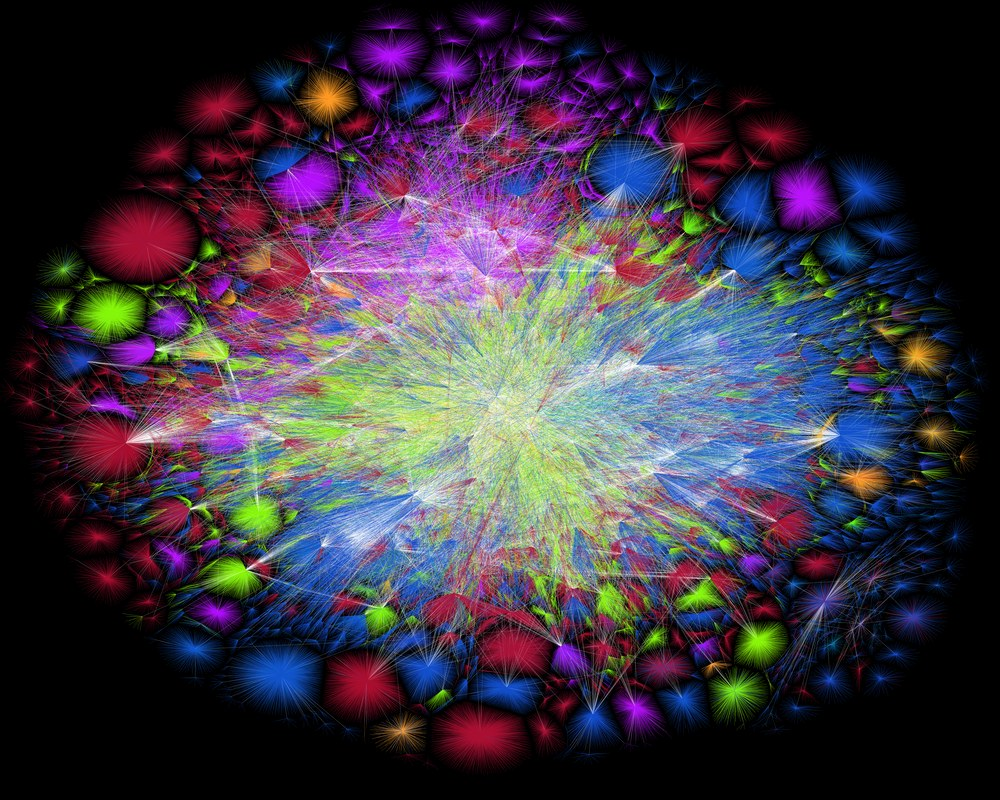
\includegraphics[width=\linewidth]{images/cover}}

% Variables & constants definitions:
\newcommand{\appname}{\texttt{userApplication}}
\newcommand{\scriptname}{\texttt{extract-codes.py}}
\newcommand{\plotscriptname}{\texttt{graphs.py}}
